W trakcie projektowania interfejsu użytkownika (UI) kluczowe jest osiągnięcie równowagi pomiędzy estetyką a funkcjonalnością. Oprócz estetycznego designu, priorytetem jest stworzenie interfejsu, który jest intuicyjny i efektywny dla użytkowników. Proces ten obejmuje systematyczne testowanie i uwzględnianie opinii, dążąc do idealnego połączenia atrakcyjnego wyglądu z praktycznym zastosowaniem, co sprawia, że interfejs nie tylko przyciąga uwagę, ale także doskonale spełnia potrzeby użytkowników.

\subsubsection{Tworzenie logo naszej gry}
Na wstępie skoncentrujmy się na kreowaniu głównego logo naszej gry, bowiem jest to nie tylko centralny element, ale także jedno z zadań, które mimo swojej doniosłości, należy do tych bardziej dostępnych w kwestii realizacji.

Rozpoczniemy od procesu projektowania, który skupi naszą uwagę na stworzeniu identyfikacyjnego znaku graficznego gry. Traktując to jako priorytetowe zadanie, pragniemy nadać mu zarówno wyjątkowość, jak i łatwą rozpoznawalność. Celem jest opracowanie logo, które nie tylko odda charakter naszej gry, ale także wyróżni ją spośród innych.

W pierwszym etapie zwrócimy szczególną uwagę na koncepcję graficzną, starając się połączyć estetykę z funkcjonalnością. Zależy nam na tym, aby logo nie tylko zachwycało wizualnie, ale również komunikowało istotne elementy związane z tematyką gry. Podejdziemy do tego zadania z pełnym zaangażowaniem, starając się wykorzystać prostotę w projektowaniu, co z kolei sprawi, że logo będzie łatwo zapamiętywalne i zrozumiałe dla potencjalnych graczy.

W procesie tworzenia skoncentrujemy się na doskonałym dopasowaniu kolorów, kształtów i czcionek, aby osiągnąć optymalny efekt wizualny. Stworzymy coś nie tylko estetycznego, ale także trwałego i godnego reprezentowania gry na rynku.

W skrócie, celem jest opracowanie nie tylko logo, ale prawdziwej ikony charakteryzującej naszą grę, która będzie zarówno atrakcyjna wizualnie, jak i funkcjonalna w przekazywaniu istotnych informacji o produkcie.

\begin{center}
{\bfseries Główne logo}
\end{center}
\begin{figure}[h]
    \centering
    
\includegraphics[scale=15]{Images/logo.png}
    \caption{Główne logo, w którym są nawiązania do tytułu tworzonej przez nas gry}
\end{figure}
\FloatBarrier

W centralnym punkcie kompozycji wyróżnia się kontur szczura, symbolicznego odniesienia do graczy na mapie, określanych w potocznym żargonie jako "szczury". Wybór tego motywu wynika z naszej koncepcji, która nawiązuje do najbardziej niebezpiecznych postaci z różnych więzień i środowisk. W świecie gry, gracz zostaje postawiony przed zadaniem eliminacji tych "szczurów", reprezentujących najbardziej zróżnicowane i złożone przestępcze postacie. Ostatecznym celem jest perfekcyjne zrealizowanie brutalnej rozgrywki, eliminując wszystkich przeciwników i upewniając się, że żaden z nich nie przeżyje starcia.
Przyjęcie motywu szczura jako symbolu podkreśla nie tylko surowość środowiska przedstawionego w grze, ale także wprowadza unikalny aspekt, który stanowi istotny element narracyjny. Szczury, jako metafora najbardziej zaciekłych przeciwników, dodają głębię fabularną oraz wywołują emocje związane z koniecznością pokonania skomplikowanego i nieprzewidywalnego przeciwnika.

W rezultacie, widoczna sylwetka szczura na głównym planie nie tylko stanowi element graficzny, ale także istotny komponent narracyjny, wzbogacający doświadczenie gracza poprzez ukazanie surowości oraz wyzwania, jakie stawia przed nim świat gry.\\

\subsubsection{Tworzenie logo Menu głównego}

Po stworzeniu głównego logo gry skoncentrujemy się na opracowaniu grafiki do menu głównego. W tym procesie zwrócimy szczególną uwagę na aspekty wizualne, aby logo doskonale wpasowało się w ogólny wygląd i tematykę gry. Naszym celem jest nie tylko estetyczna prezentacja w menu, ale także harmonijne zintegrowanie logotypu, tworząc spójną wizualną całość. Poprzez analizę detali kompozycji, kolorów i proporcji, dążymy do uzyskania efektu, który przyciągnie uwagę graczy i skutecznie przekazywać będzie charakter gry. Proces ten obejmie staranne dostosowanie grafiki do kontekstu menu, tworząc przyjemne wrażenie wizualne już na pierwszym spotkaniu gracza z grą.
\begin{center}
\end{center}
\begin{figure}[h]
    \centering
    
\includegraphics[scale=0.2]{Images/mainLogo.jpg}
    \caption{Logo w głównym Menu, domyślnie jest z przezroczystym tłem (w tym przypadku tło dodane po ukończeniu logo)}
\end{figure}

Na przedstawionej grafice zauważamy, że logo zostało zręcznie wkomponowane jako litera w tytule gry. Ten subtelny zabieg nie tylko stanowi estetyczny atut dla oka, ale także wyróżnia się doskonałą czytelnością, nie dominując nad pozostałymi elementami. Stworzone w ten sposób logo idealnie komponuje się z ogólnym układem graficznym, prezentując równowagę między atrakcyjnym wyglądem a funkcjonalnością.

W trakcie tworzenia menu głównego gry planujemy skorzystać z tego logo, umieszczając je w sposób, który będzie sprzyjał spójności i łatwości odczytu dla graczy. Intencją jest stworzenie Main Menu, które nie tylko będzie wizualnie atrakcyjne, ale również praktyczne, umożliwiając płynną nawigację i dostarczając przyjemnego doświadczenia użytkownika od samego początku interakcji z grą.\\

\subsubsection{Main Menu}
Nadszedł moment, aby przystąpić do projektowania menu głównego naszej gry. W tym celu stworzyliśmy wstępny, aczkolwiek szczegółowy szkic, korzystając z popularnych narzędzi graficznych. Ten etap obejmuje opracowanie koncepcji, układu i funkcji, które będą dostępne dla gracza na etapie rozpoczęcia gry. Stworzyliśmy schematyczny rysunek, który stanowi swoiste mapowanie wizualne tego, jak zamierzamy zorganizować interakcję użytkownika z grą, uwzględniając zarówno estetyczne aspekty, jak i praktyczne potrzeby użytkowników.

W tym procesie zwracamy uwagę na czytelność, intuicyjność nawigacji oraz estetyczne dopasowanie do ogólnej koncepcji gry. Wszystko to ma na celu stworzenie menu głównego, które nie tylko przyciągnie uwagę graczy swoim wyglądem, ale również zapewni im łatwą i satysfakcjonującą interakcję z grą od samego początku.

\begin{figure}[h]
\begin{center}
{\bfseries Rysunek schematyczny menu}
\end{center}
    \centering
    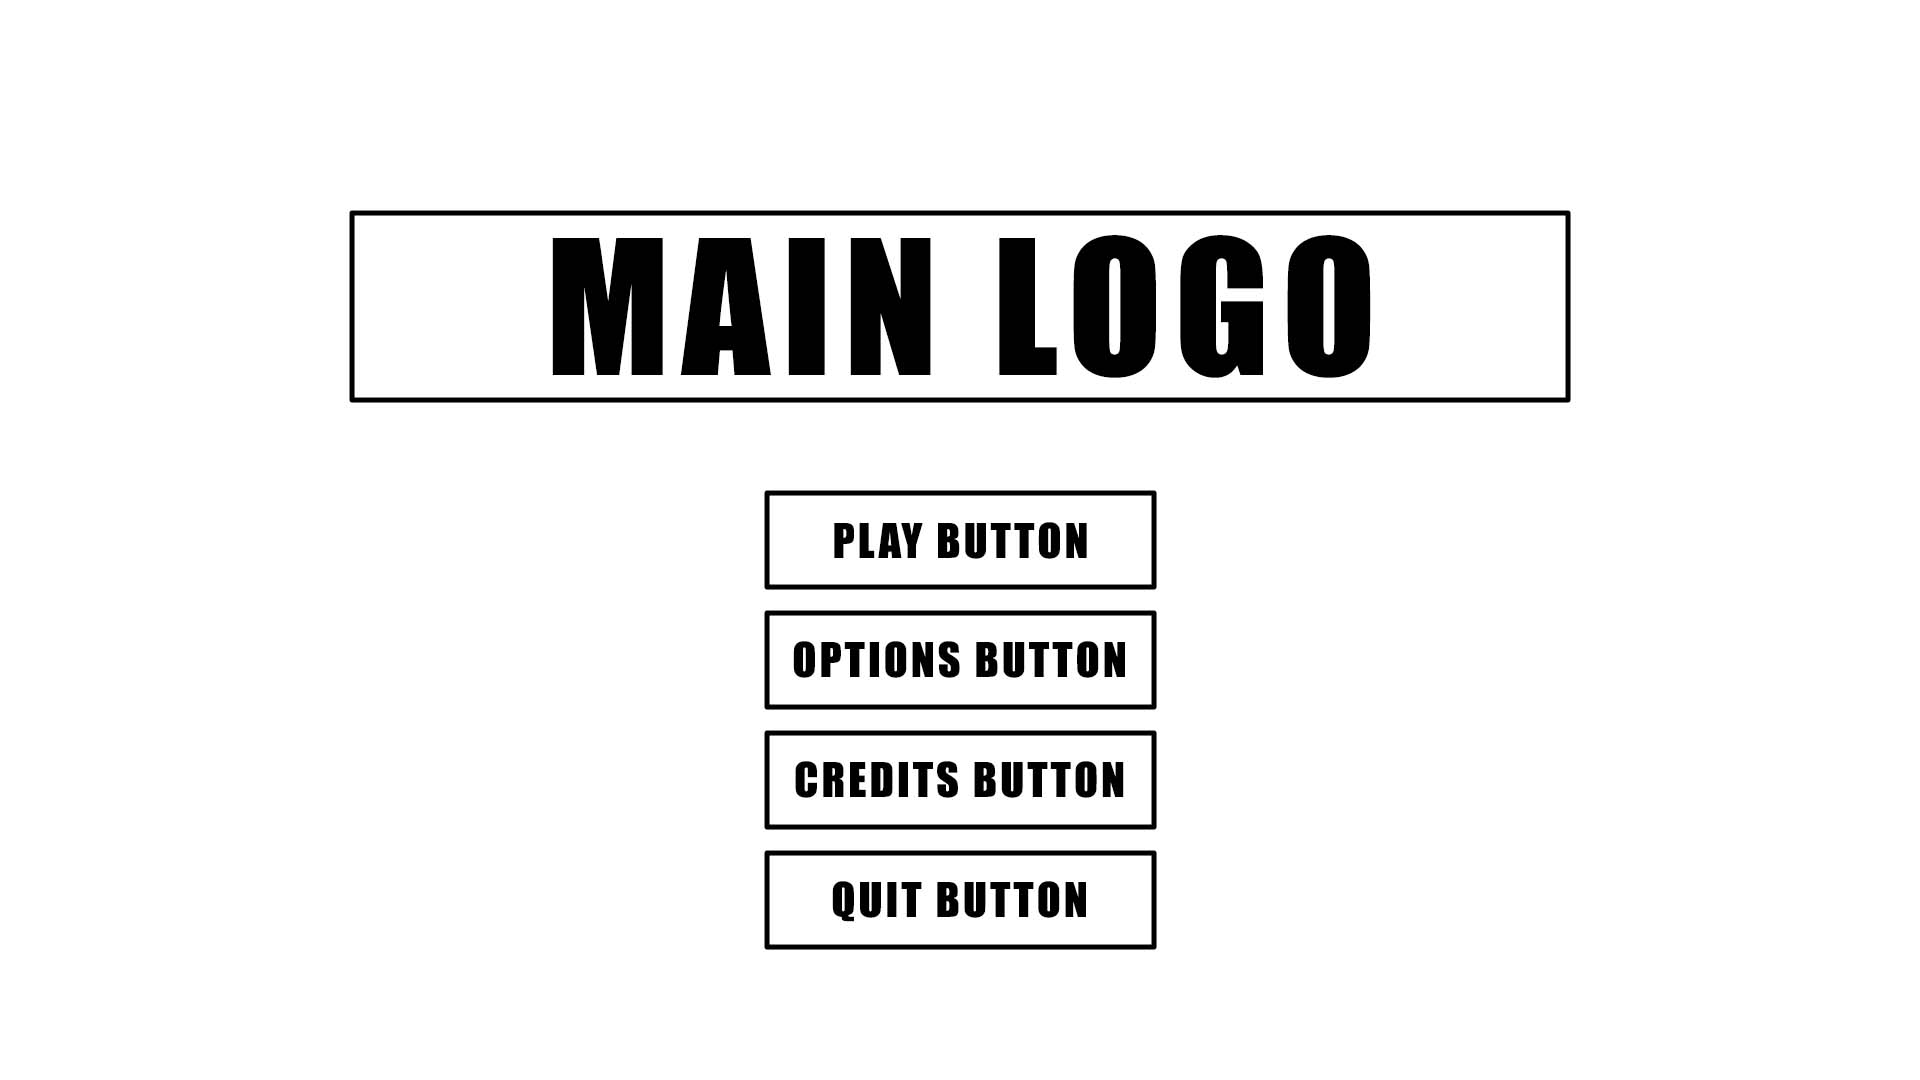
\includegraphics[scale=0.2]{Images/templateMenu.jpg}
    \caption{Na powyższym obraz możemy zobaczyć bardzo uproszczony rysunek schematyczny z procesów tworzenia Menu}
\end{figure}
\FloatBarrier

Po akceptacji wszystkich członków teamu możemy zacząć tworzenie naszego projektu w grze.

\begin{figure}[h]
\begin{center}
{\bfseries Gotowe Main Menu - w grze}
\end{center}
    \centering
    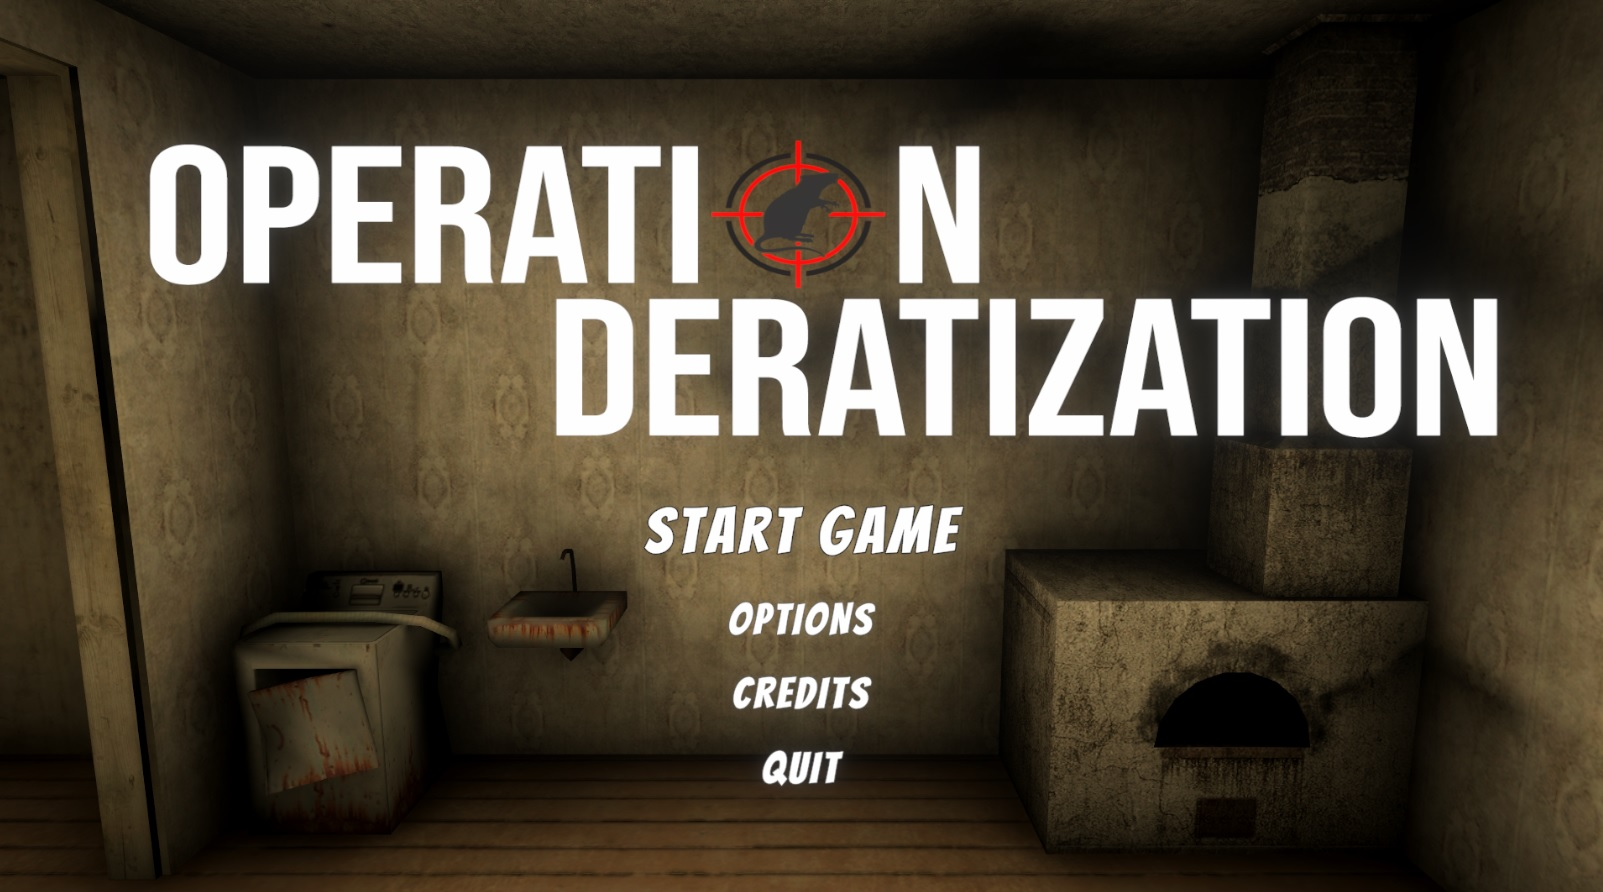
\includegraphics[width=0.75\linewidth]{Images/mainMenuInGame.jpg}
    \caption{Nasze Main Menu utworzone już w grze}
\end{figure}
\FloatBarrier

Tworzenie zaczynamy od zrobienia sceny, na której ustawiliśmy dom, w którym znajduje się całość naszego Menu. Wokół postawiliśmy drzewa, które pełnią formę estetyczną, ponieważ wszystko widać przez okna a nie chcemy aby była widoczna pusta przestrzeń. Następnie w naszym budynku planujemy i tworzymy wnętrze, dodajemy kilka assetów aby nie świeciło ono pustkami. Jak możemy zobaczyć sugerowaliśmy się naszym wcześniej pokazywanym rysunkiem schematycznym. W górnej części widnieje zaprojektowane logo wraz z tytułem gry, natomiast poniżej funkcjonalne przyciski, które odpowiadają przypisanym im funkcjom. Dodatkowo pozwoliliśmy sobie dodać osobną planszę wraz z wyróżnieniem twórców gry znajdującą się pod przyciskiem "credits".\\

\begin{figure}[h]
\begin{center}
{\bfseries Credits - w grze}
\end{center}
    \centering
    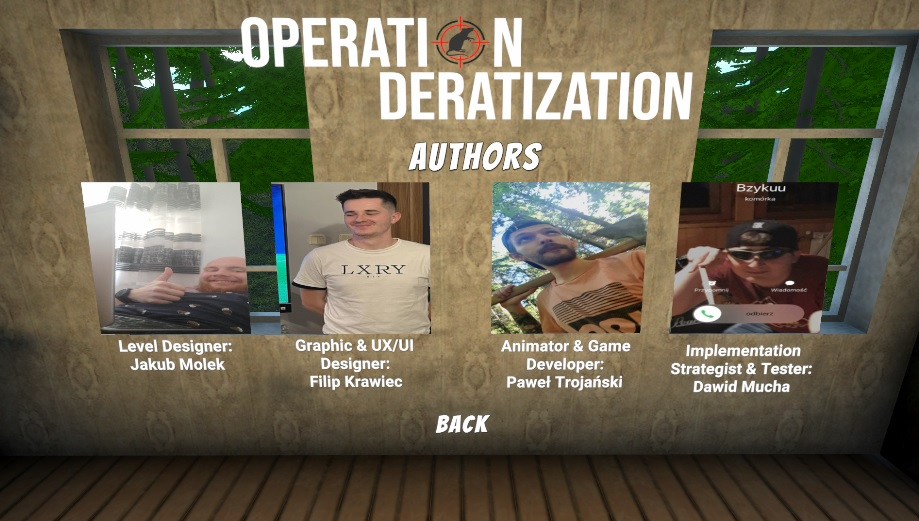
\includegraphics[width=0.75\linewidth]{Images/CreditsInGame.jpg}
    \caption{Plansza "Credits"}
\end{figure}

Jak możemy zobaczyć na powyższym obrazku plansza "Credits" zawiera informacje o autorach gry. W tle możemy zobaczyć wcześniej wspominane drzewa, które elegancko wypełniają na pustą przestrzeń na terenie przygotowanym pod Main Menu, w górnej części możemy zobaczyć również logo, które występuje w głównej planszy Menu. Poniżej znajdują się zdjęcia wraz z danymi autorów oraz w postaci dodatkowego smaczka mamy także przypisane do nich odpowiednie role przy tworzeniu gry. przyciskiem "Back" znajdującym się na dole strony wracamy do głównej planszy naszego menu, gdzie możemy wejść w opcje naszej gry bądź z niej wyjść.\\

\begin{figure}[h]
    \begin{center}
    {\bfseries Options - w grze}
    \end{center}
    \centering
    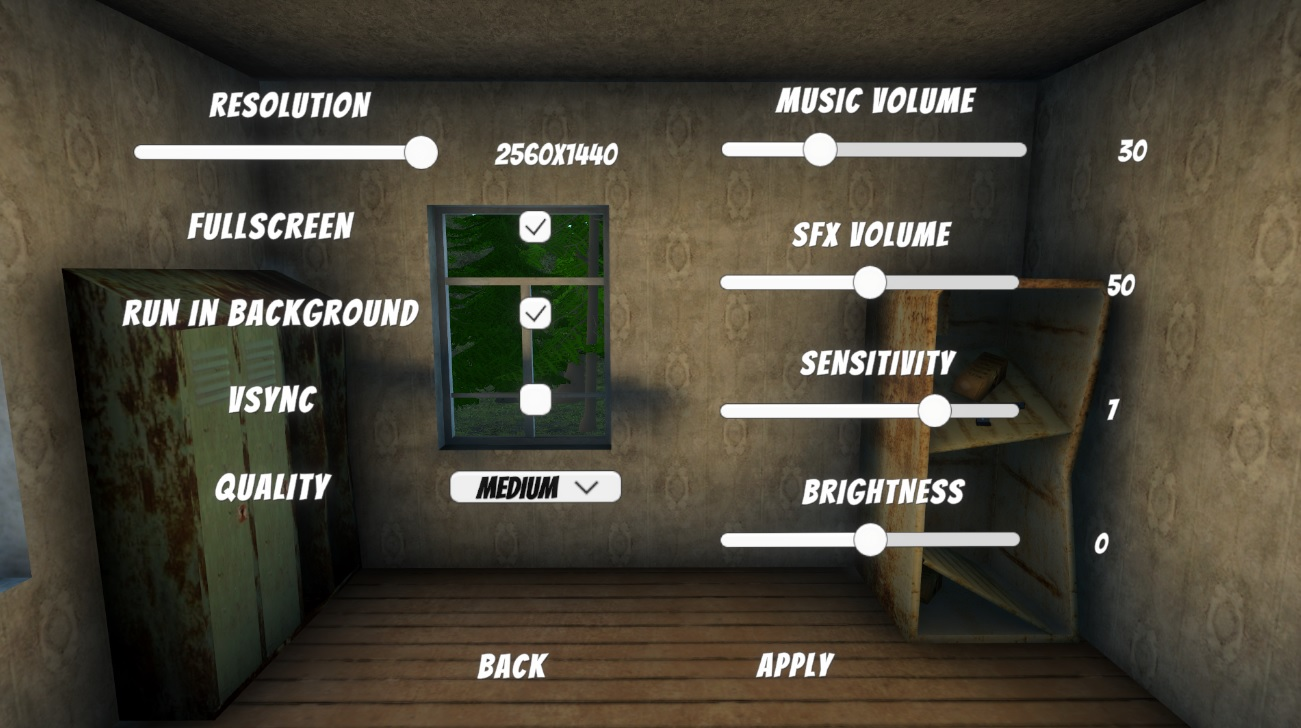
\includegraphics[width=0.75\linewidth]{Images/menuUpdated.jpg}
    \caption{Plansza "Options"}
    \begin{flushleft}
    Kolejną pozycją na naszej liście przycisków są opcje gry. Tutaj możemy zmienić wiele aspektów naszej gry, począwszy od wersji graficznej, przechodząc do akustycznej i kończywszy na indywidualnych preferencjach ustawień takich jak czułość czy używanie pełnego ekranu. Poniżej znajdują się dwa przyciski, po naciśnięciu przycisku \textit{Apply} wyskakuje nam okienko potwierdzenia (czy na pewno chcemy zapisać ustawienia gry), oraz po naciśnięciu przycisku \textit{Back}, tak jak w poprzednim przypadku cofamy się do głównej planszy naszego Menu.\\
    \end{flushleft}
\end{figure}
\FloatBarrier
\begin{figure}[h]
\begin{center}
{\bfseries Quit - w grze}
\end{center}
    \centering
    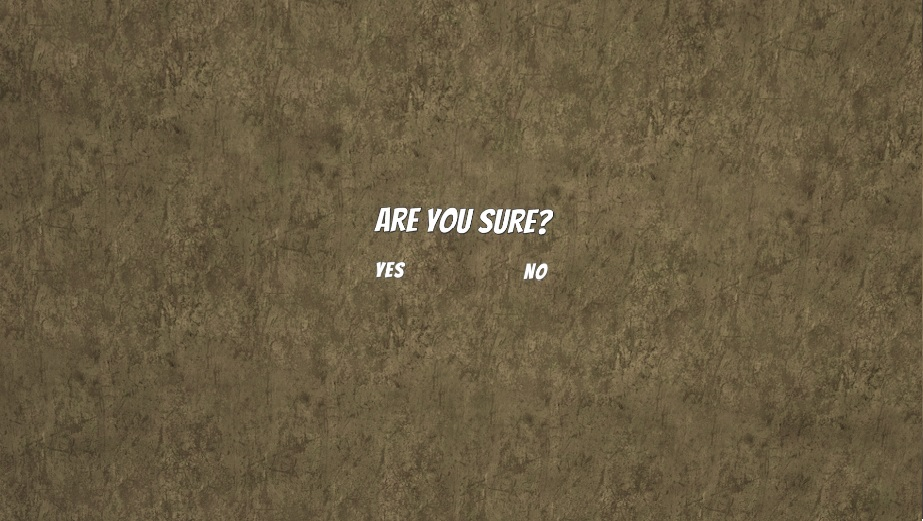
\includegraphics[width=0.75\linewidth]{Images/QuitInGame.jpg}
    \caption{Plansza "Quit"}
\end{figure}
\FloatBarrier

Jest to jedna z najprostszych i najbardziej podstawowych plansz w naszym Menu głównym. Jej zadaniem jest upewnić się czy gracz jest pewien swojej decyzji w stu procentach. Znajdują się na niej dwa przyciski \textbf{\textit{Yes}} oraz \textbf{\textit{No}}. jak możemy się domyślać po wciśnięciu przycisku po lewej stronie, nasza gra zostanie zamknięta i przejdziemy do swojego pulpitu. Ciekawostka ten ekran także jest wykorzystywany do zapisywania ustawień z planszy "Options", o której mowa była we wcześniejszym opisie.\\

\subsubsection{Loading Screen}
Jeżeli chodzi o sam \textbf{\textit{"Loading Screen"}}, pojawiającym się np. pomiędzy Menu a samą grą. Rozpoczęliśmy od przeglądnięcia ekranów wczytywania z rozmaitych gier i na tej podstawie stworzyliśmy nasz autorski projekt.

\begin{figure}[h]
\begin{center}
{\bfseries InGame Loading Screen}
\end{center}
    \centering
    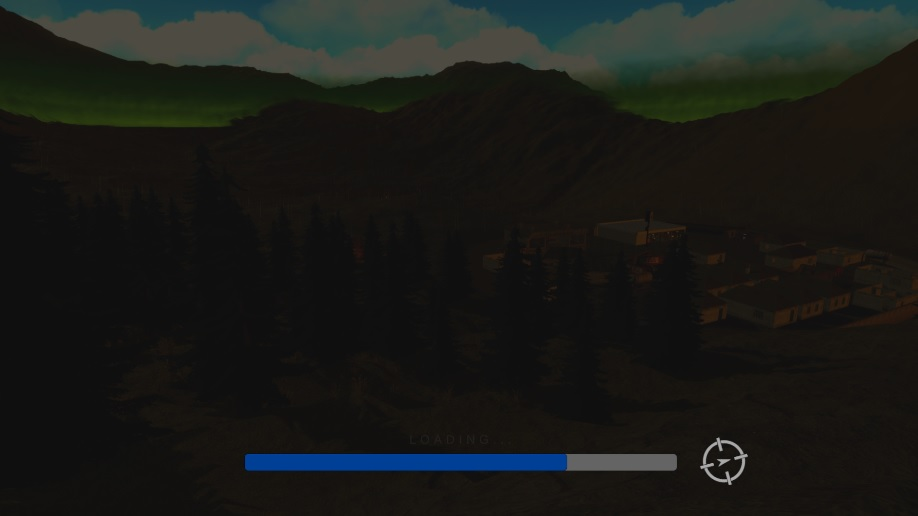
\includegraphics[width=0.75\linewidth]{Images/LoadingScreenIngame.jpg}
    \caption{Loading Screen po zaprojektowaniu i wykonaniu}
\end{figure}
\FloatBarrier

Jak możemy zobaczyć jest to jeden z podstawowych Loading Screenów. Znajduje się na nim pasek (w tym przypadku w trakcie ładowania, po prawej od paska oraz nad nim znajdują się animowany napis oraz animowana ikona naszego Trackera. W tle dodatkowo przedstawiona jest mapa, na której możemy zobaczyć przedsmak tego co się znajduje w głównej grze.

\subsubsection{InGame Pause Menu}
Istotnym elementem w doświadczeniu gracza jest "InGame Pause Menu", które można otworzyć za pomocą przycisku ESC. To istotne narzędzie zapewniające dostęp do szeregu opcji bezpośrednio w trakcie rozgrywki. W ramach tego menu, gracz ma możliwość wyjścia do menu głównego, zrestartowania rozgrywki oraz wejścia do "Ingame Options Menu". Ostatnie z wymienionych menu umożliwia dokonywanie zmian w ustawieniach gry, bez konieczności przerywania aktualnej rozgrywki.

Warto jednak zauważyć, że po wejściu do "InGame Pause Menu" gra może ulec chwilowemu zatrzymaniu, co zapewnia bezpieczne i spokojne środowisko do dokonywania zmian w ustawieniach bez pośpiechu. Ten krótkotrwały "freeze" gry jest integralną częścią procesu i zapewnia stabilność operacji dokonywanych w trakcie korzystania z "InGame Pause Menu". Dzięki tej funkcji, gracz ma pewność, że wszelkie zmiany w ustawieniach odbywają się w kontrolowany sposób, nie zakłócając płynności rozgrywki.

\begin{figure}[h]
\begin{center}
{\bfseries InGame Pause Menu}
\end{center}
    \centering
    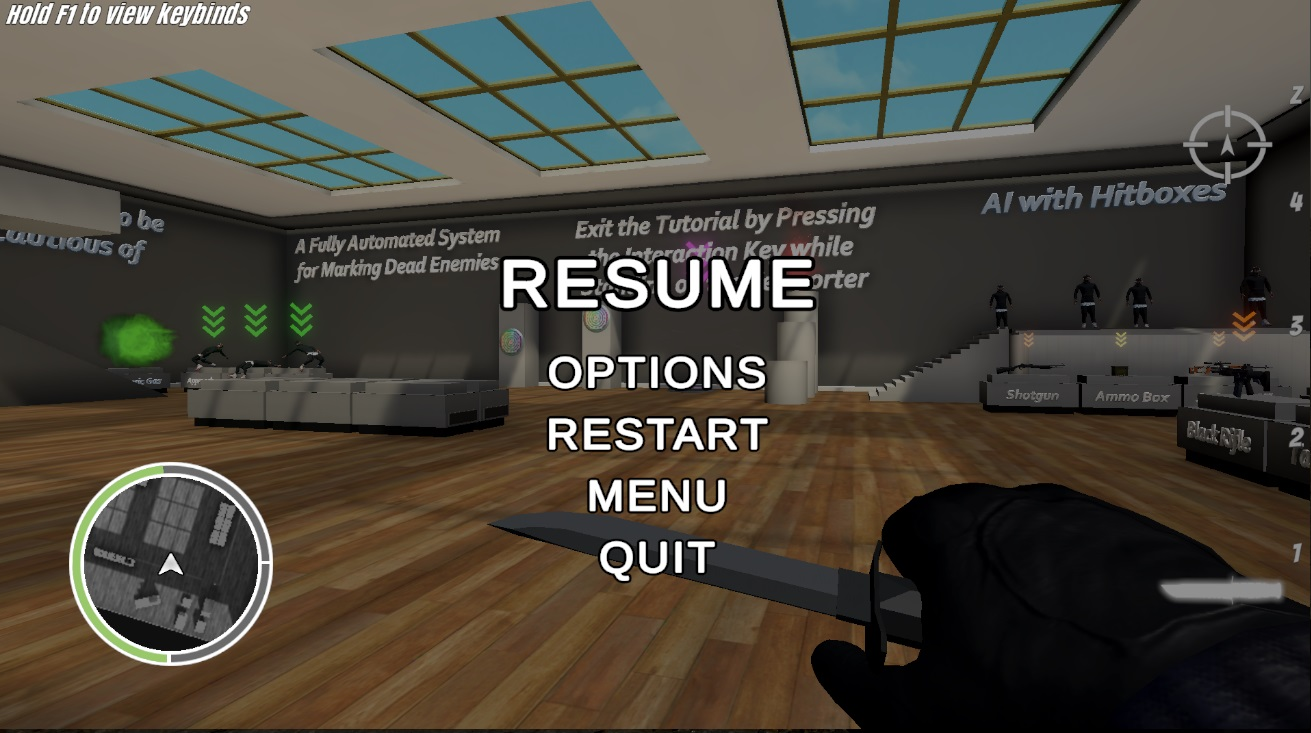
\includegraphics[width=1\linewidth]{Images/menuIngameupdated2.jpg}
        \caption{InGame Pause Menu po zaprojektu i utworzeniu}
    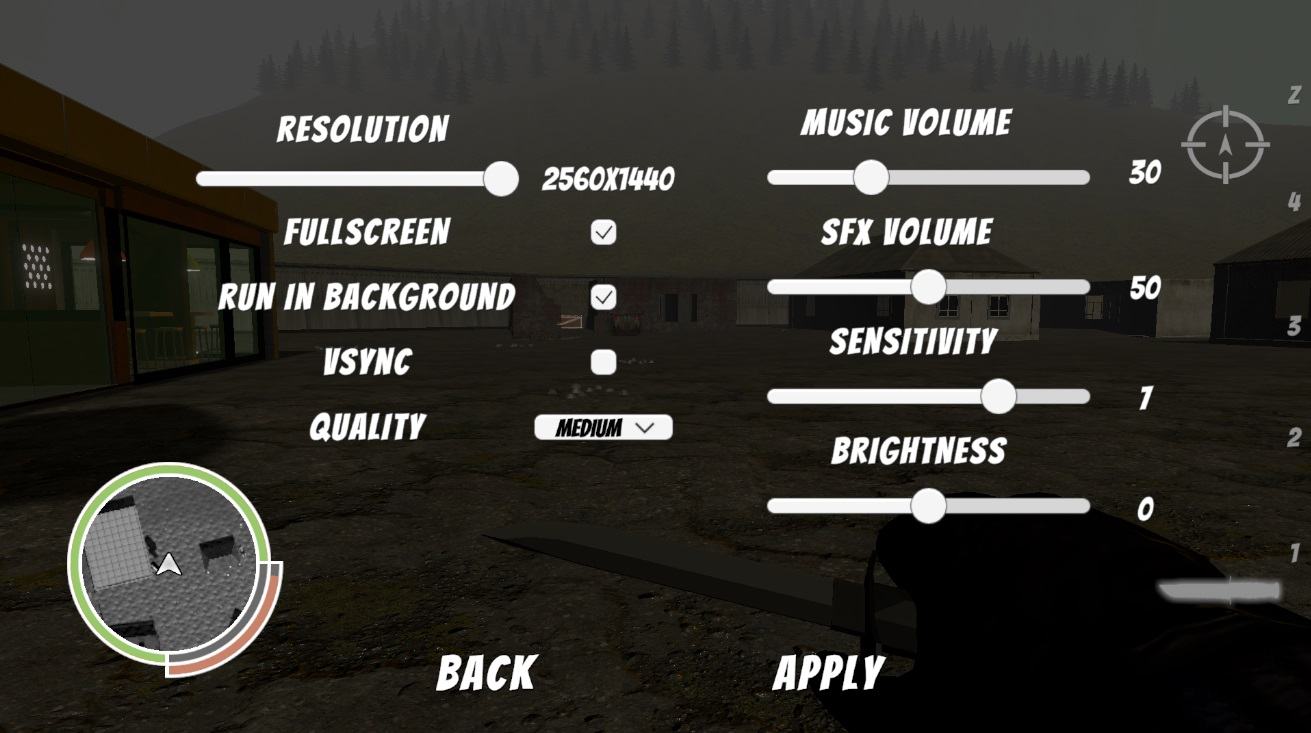
\includegraphics[width=1\linewidth]{Images/menuIngameUpdated.jpg}
    \caption{InGame Options Menu po zaprojektu i utworzeniu}
\end{figure}
\FloatBarrier

\subsubsection{Grafiki wykorzystane do Cutscenek}

Wspomniane CutSceny, czyli sekwencje filmowe w grach, stanowią niezwykle istotny element w kreowaniu bogatego narracyjnego doświadczenia. Na specjalne życzenie jednego z naszych animatorów, podjęliśmy się stworzenia kilku "memowych grafik", które stanowią kreatywną odmianę tego konwencjonalnego aspektu. Poniżej znajdują się zdjęcia przedstawiające te unikatowe grafiki, które zostały zrealizowane z myślą o dodaniu elementu humorystycznego i nieformalnego charakteru do świata gry.

Rozwinięta kreatywność w obszarze CutScen sprawia, że gracze mogą doświadczać nie tylko bogatej narracji, ale także elementów zabawy i humoru. Memowe grafiki stanowią oryginalne podejście do tego, co często bywa traktowane poważnie, dodając unikalny, lekki akcent do animacji. To przykład, jak z dbałością o detale podejście do tworzenia rozrywki może wprowadzić nową, niekonwencjonalną jakość do gier.

\begin{figure}[h]
\begin{center}
{\bfseries Cutscenes graphic}
\end{center}
    \centering
    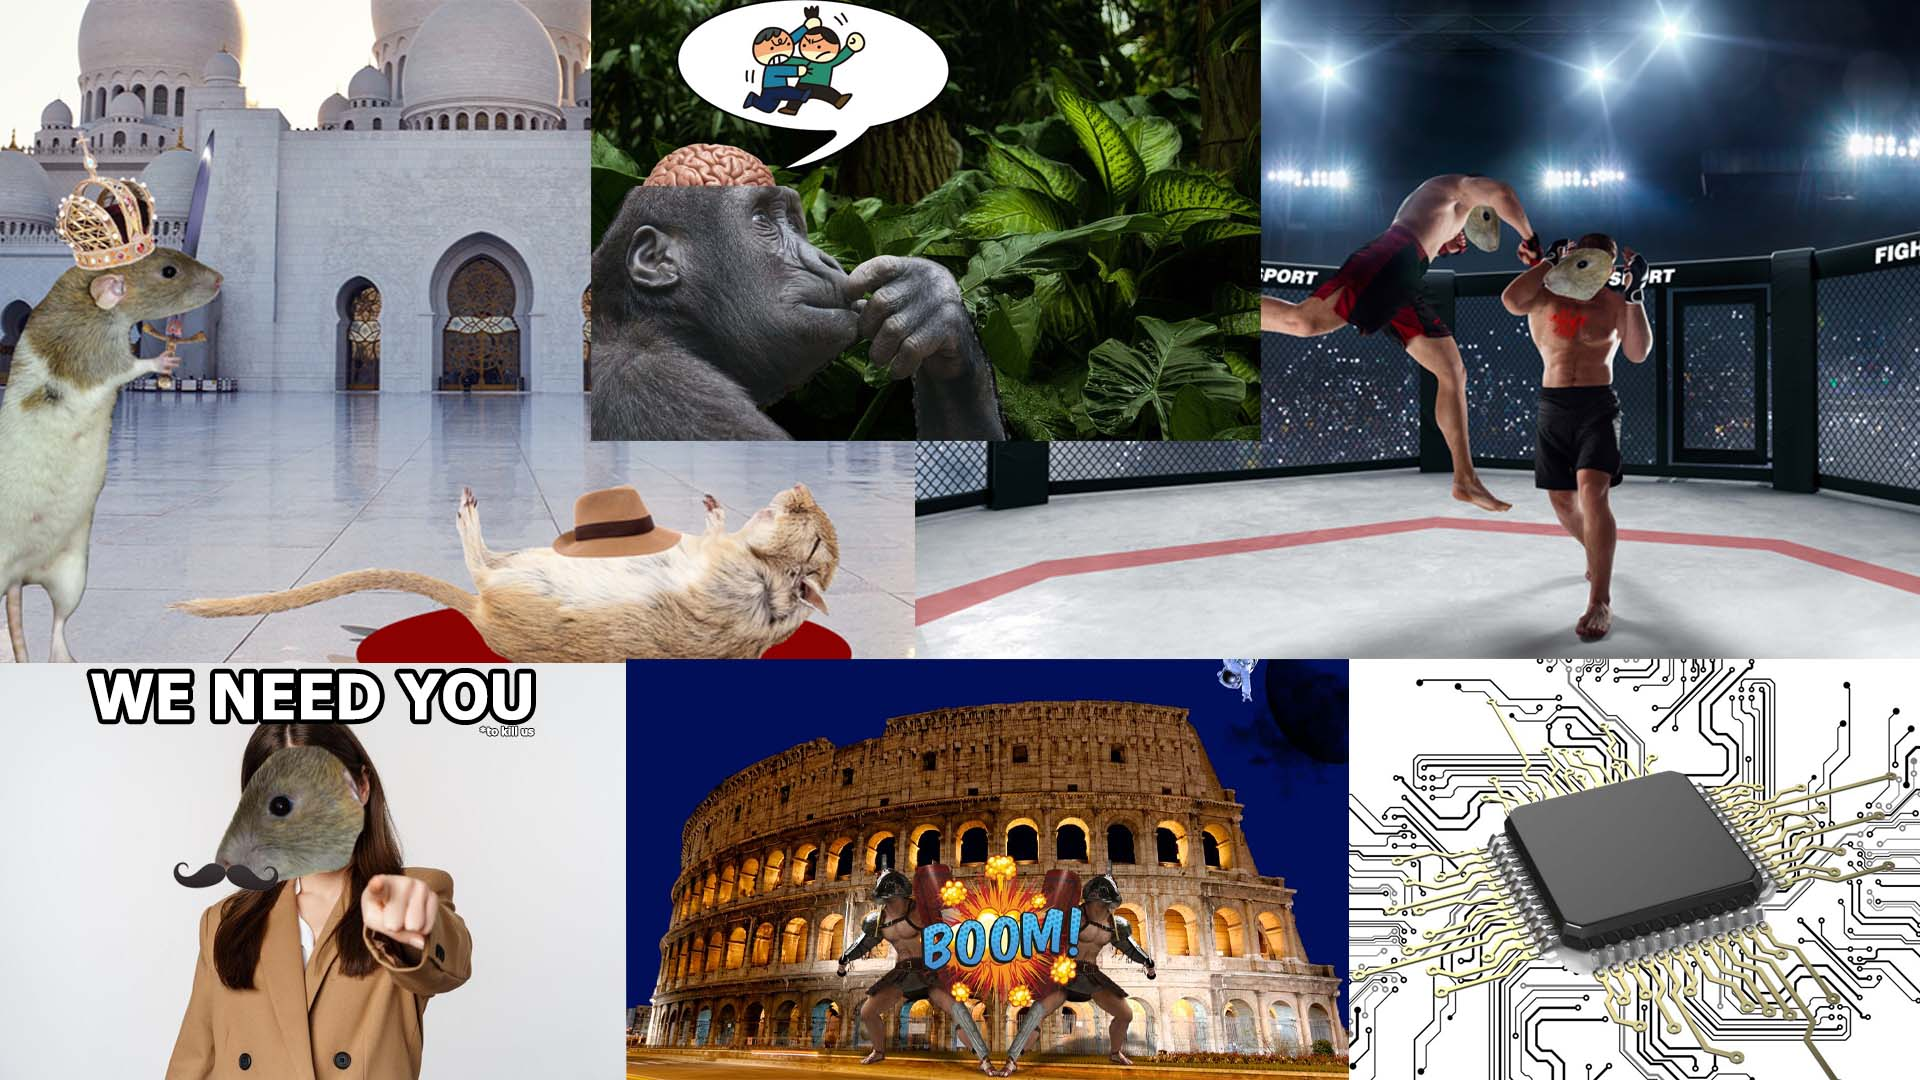
\includegraphics[width=1\linewidth]{Images/wszystkie grafiki.jpg}
        \caption{Grafiki użyte w cutscenach}
\end{figure}
\FloatBarrier
